%SOURCE : https://github.com/Gp2mv3/Syntheses
\documentclass[fr]{sourcefiles/eplexam} % For a master exam in English, replace fr by en

%\usepackage{sourcefiles/eplcode} % Si l'examen contient du code. La commande pour insérer du code est \begin{lstlisting} ou pour un fichier \lstinputlisting{nomDeFichier}
%\lstset{language={Oz}, morekeywords={for,do,lazy}} % exemple de réglage avec Oz

\usepackage{xcolor}
\usepackage{listings}
\definecolor{vgreen}{RGB}{104,180,104}
\definecolor{vblue}{RGB}{49,49,255}
\definecolor{vorange}{RGB}{255,143,102}

\lstdefinestyle{verilog-style}
{
    language=Verilog,
    basicstyle=\small\ttfamily,
    keywordstyle=\color{vblue},
    identifierstyle=\color{black},
    commentstyle=\color{vgreen},
    numbers=left,
    numberstyle=\tiny\color{black},
    numbersep=10pt,
    tabsize=8,
    literate=*{:}{{\textcolor{black}{:}}}1
}

\newcommand\colorIndex[1]{[\textcolor{vorange}{#1}]}


\usepackage{makecell}
\renewcommand\theadalign{bc}
\renewcommand\theadfont{\bfseries}
\renewcommand\theadgape{\Gape[4pt]}
\renewcommand\cellgape{\Gape[4pt]}




\graphicspath{{img/}}

\hypertitle{Synthesis of digital integrated circuits}{7}{ELEC}{2570}{2022}{Janvier}{All} % Remplacer Majeure par All si ce n'est pas un cours à option
{Maxime Leurquin}
{David Bol}

%Ce template a pour but de faciliter la rédaction des examens destinés à être posté sur Github. Cependant, il ne peut être posté sans respecter la hiérarchie établie dans le dossier du drive. Il est donc nécessaire de passer par un administrateur du drive (contact.epldrive@gmail.com), ou en suivant les instructions détaillées dans le fichier "How_to_Contribute" sur https://github.com/Gp2mv3/Syntheses. Notez qu'il est possible de contribuer de diverses manières!


%La ligne suivante est à supprimer à la compilation! Cette ligne crée une erreur, mais a été ajoutée afin d'éviter qu'overleaf ne mette du rouge partout.
\begin{document}

\noindent We had 3h to finish the exam but almost everyone finished in 2h. The exam was worth 14 points and the weekly assignments were worth 6 points. The exam was closed book.

\section{Semiconductor business}
\begin{enumerate}
    \item Why has the design cost of SoCs increased over the last decades? Consider a typical product type such as microprocessors.
    \item  How does the industry generate a financial return on this high design cost of SoCs?
\end{enumerate}
\nosolution


\section{Verification}
\begin{enumerate}
    \item  Give an example of a static verification method used in the course project.
    \item Give an example of a dynamic verification method used in the course project.
\end{enumerate}
\nosolution



\section{Embedded programming and low-power design}
\begin{enumerate}
    \item What is interrupt-driven programming?
    \item Compared to polling-based programming, how can we use it to save power in the pillcam image compression application of the project, in case the compression of an image would be completed before the CMOS imager has the next image ready? Explain with a graph of the power consumption over time.
\end{enumerate}
\nosolution

\section{Robust HDL}
\noindent A digital IC containing the Verilog code portion below is not functional. Why? How can we solve the issue?
\begin{lstlisting}[style={verilog-style}]
// HDL Verilog code leading to a non functional digital IC.
reg [31:0] haddr_last = 32d'0;

...

//Record AHB transaction information
always @(posedge CLK) begin
    haddr_last <= HADDR;
end
\end{lstlisting}

\begin{solution}
Fixing a value to a register outside of an \verb|always| statement is a little bit like an initial statement. It is not synthetisable.
\begin{lstlisting}[style={verilog-style}]
// Functionnal HDL Verilog code
reg [31:0] haddr_last;

...

//Record AHB transaction information
always @(posedge CLK, posedge RST) begin
    if(RST==1):
        haddr_last <= 32d'0;
    else:
        haddr_last <= HADDR;
end
\end{lstlisting}
\end{solution}


\section{Design clocking}
\begin{enumerate}
    \item What is metastability in the context of clock domain crossing? Use a timing diagram to illustrate the phenomenon.
    \item  In case of metastability, what is the consequence on circuit operation?
    \item How do we prevent metastability to disrupt circuit operation?
\end{enumerate}
\nosolution


\section{Memory architecture}
\begin{enumerate}
    \item What is the mux factor in an embedded memory hard macro?
    \item  What is the read access time (RAT) of an embedded memory hard macro?
    \item How is the RAT affected by the memory mux factor? Why?
\end{enumerate}
\nosolution


\section{ Physical implementation}
\noindent Fig. \ref{floorplans} shows two floorplans with a different core row utilization. What are the pros and cons of the floorplan with high-utilization on the left?

\begin{figure}[h]
    \centering
    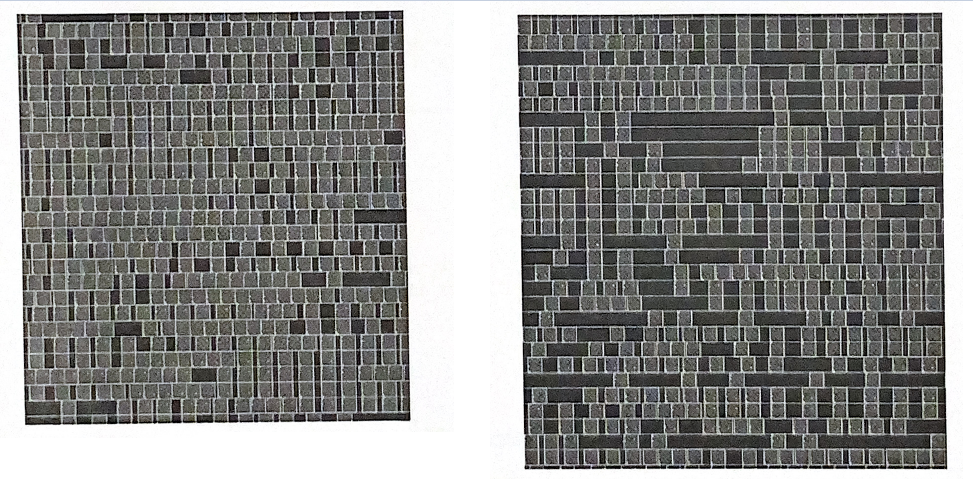
\includegraphics[width=0.8\textwidth]{FloorplansQ7.png}
    \caption{Floorplans with different core row utilization}
    \label{floorplans}
\end{figure}


\begin{solution}
\begin{itemize}
    \item In the floorplan with low utilisation there is less congestion between the cells, and thus the tool will be able to do the routing easier. Furthermore if there is a timing problem the tool will be able to make timing optimisations as there is space left to add logic or change routes.
     \item In the floorplan with high utilisation the routing is shorter, and the wires will be shorter.
\end{itemize}






\end{solution}


\section{Technology scaling}
\begin{enumerate}
    \item How does technology scaling impact the routing delay of global wires (from one end of the chip to the other)? Why?
    \item Give a solution at the technology level. 
    \item Give a solution at the circuit design level. Explain your answers.
\end{enumerate}
\nosolution

\section{DSP}
\noindent How many cycles, PMEM and DMEM accesses do we need to compute one output sample of an Ntap FIR filter with a Von Neumann general-purpose processor (GPP)? Justify your answer with a pseudo assembly code.
\begin{solution}
8N cycles in total: 6N for the PMEM accesses, and 2N for the DMEM accesses.
N-tap FIR filter example: 
$$y(n)=\sum^{N-1}_{i=0}c(i)\cdot x(n-i)$$

\begin{lstlisting}[style={verilog-style}]
//register allocation
// R0:i   R1:x(n-i)   R2:c(i)   R3:y(n) 
// R4:addr[x(n-N)]  R5addr[c(N)]

//initialisation
...
//loop
LOAD R1 <- [R4,R0]   
LOAD R2 <- [R5,R]   
MULT R1 <- R1,R2
ADD R3  <- R1,R3
SUB R0  <- R0, #1
BNE     R0,#0  

//termination
STORE   R3->y(n)
\end{lstlisting}

\end{solution}

\pagebreak
\section{ROM memory (based on the course project)}
\noindent We consider the baseline PixRacer SoC as used in the course project clocked at $50 \mathrm{MHz}$ using two $32$kB SRAM macros for program and data memories. Fig. \ref{fig:projectP1} shows the synthesis power report during JPEG-XS compression.

\begin{figure}[h]
    \centering
    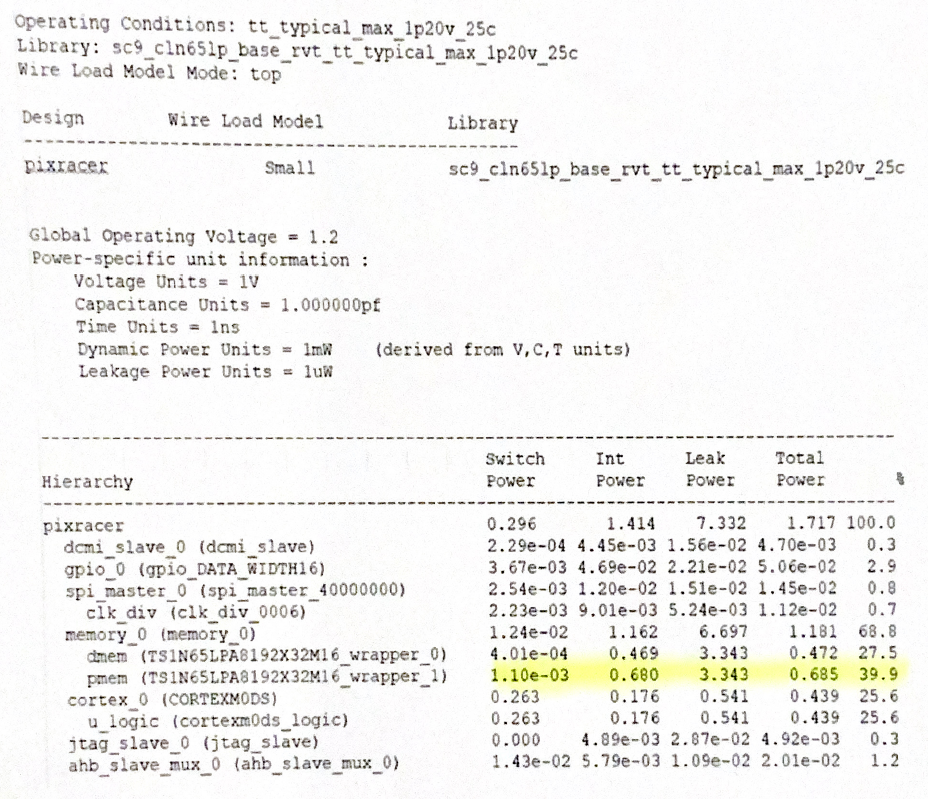
\includegraphics[width=\textwidth]{projectQuestionP1.png}
    \caption{Synthesis power report with only SRAM macros}
    \label{fig:projectP1}
\end{figure}

\noindent In order to avoid reprogramming the endoscopic pill camera at each utilization, we would like to replace the SRAM memory macro where the program instructions are stored, by a ROM memory macro embedded directly in the PixRacer SoC. In the target $65 \mathrm{~nm}$ CMOS technology, we have access to a single $32$kB ROM macro configuration, whose PPA are given in Table \ref{table1}, as compared to the SRAM macro.

\begin{figure}[h]
    \centering
    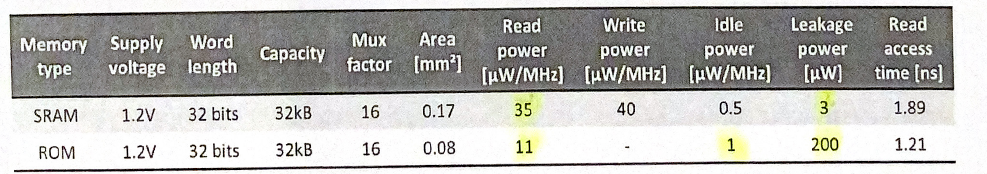
\includegraphics[width=0.8\textwidth]{ProjectQuestionP2.png}
    \caption{PPA of the memory macros.}
    \label{table1}
\end{figure}


\begin{enumerate}
    \item Evaluate the power consumption that the SoC would have with the ROM macro used as program memory, while keeping everything else unchanged.
    \item Assuming that the IP provider company who designed the ROM macro is able to customize it, which other configuration would you request to further reduce the power consumption? Justify and explain the potential associated modifications of the SoC architecture.
\end{enumerate}

\nosolution




\end{document}

